\chapter{User Interaction and Collision Detection}

In this chapter you will incorporate User Interaction into the object catching
game. The first step will be implementing a drag and drop mechanism that lets
the user move the pot in order to catch objects. To detect if the player has
caught or missed an object we will implement basic collision detection - note
that you will later learn how to use the \cocos{} physics engine that provides
collision detection out of the box. Whether you want to implement your own
collision detection or use the physics engine will depend a lot on the type of
game you are developing and we will discuss the advantages of both approaches
throughout this book.

When we've implemented the first control scheme we will add a second option for
players - controlling the game with the accelerometer of the device, another
common way to interact with mobile games.

As a byproduct of implementing these features we will work with translating
positions and sizes between different node spaces and the world space, so we
will be discussing that important concept throughout this chapter as well.

\section{Add the pot to the game}
The goal of our game will be to move a pot across the screen and try to catch
all the vegetables while avoiding catching inedible objects. Before we can
implement the drag and drop mechanism we need to add the pot assets to our game,
we're going to do that in the \SB{} project, open it now.

Typically we use individual \ccbfile{}s for each type of object in our game,
however for this game we need to make an exception due to the specific way in
which order \cocos{} renders our objects in the game.

\subsection{Working with the z-order}\index{Z-Order}
Throughout this book we are working with a 2D engine. In a 2D engine depth can
only be represented by certain objects being placed in front or behind of other
objects. \cocos{} uses the following criteria to decide which nodes are rendered
in front of other nodes:
\begin{enumerate}
  \item Child nodes are rendered in front of their parent nodes
  \item Siblings (nodes with the same parent) are rendered in order of their
  \inlinecode{zOrder} property; nodes with higher \inlinecode{zOrder} are
  rendered in front of nodes with a lower one
  \item If two siblings have the same \inlinecode{zOrder} the siblings are
  rendered in reverse order of how they have been added (the latest added node
  is rendered in front of all other nodes)
\end{enumerate}

As you can see from the description above the \inlinecode{zOrder} only affects
how siblings are ordered, \cocos{} currently does not have a global
\inlinecode{zOrder}. For our game we want to create the illusion of objects
dropping into a pot, we can do that using the \cocos{} Z-order as shown in
the figure below. 

\begin{figure}[H]
		\centering
		
\includegraphics[width=0.9\linewidth]{images/Chapter3/drawing_order.png}
		\caption{Left: Objects on different Layers, Right: How the Z-Order influences
		on which Layer a node is rendered}
\end{figure}

For this solution to work all the falling objects and the bottom and top part of
our pot need to have the same parent node, otherwise we would not be able to use
the Z-Order to place the falling objects between the two parts of the pot. 

That is the reason why we are not creating a separate \ccbfile{} for the pot
object and instead place it inside of \inlinecode{MainScene.ccb}. There would be
other ways to work around this issue but adding the pot to the Main Scene is a
good solution for this game.

\begin{details}[frametitle={Global Z-order in \cocos{}}] 
While \cocos{} does not have support for global Z-order at the moment, it is
being discussed as a potential feature for future releases. Many games run into
issues as discussed above due to the lack of this feature. You can follow the
discussion on GitHub: \url{https://github.com/cocos2d/cocos2d-swift/issues/662}.
\end{details}

\subsection{Setting up the pot assets}
Equipped with everything we need to know about Z-order let's add the pot assets
to our Main Scene in \SB{}:

\begin{figure}[H]
		\centering
		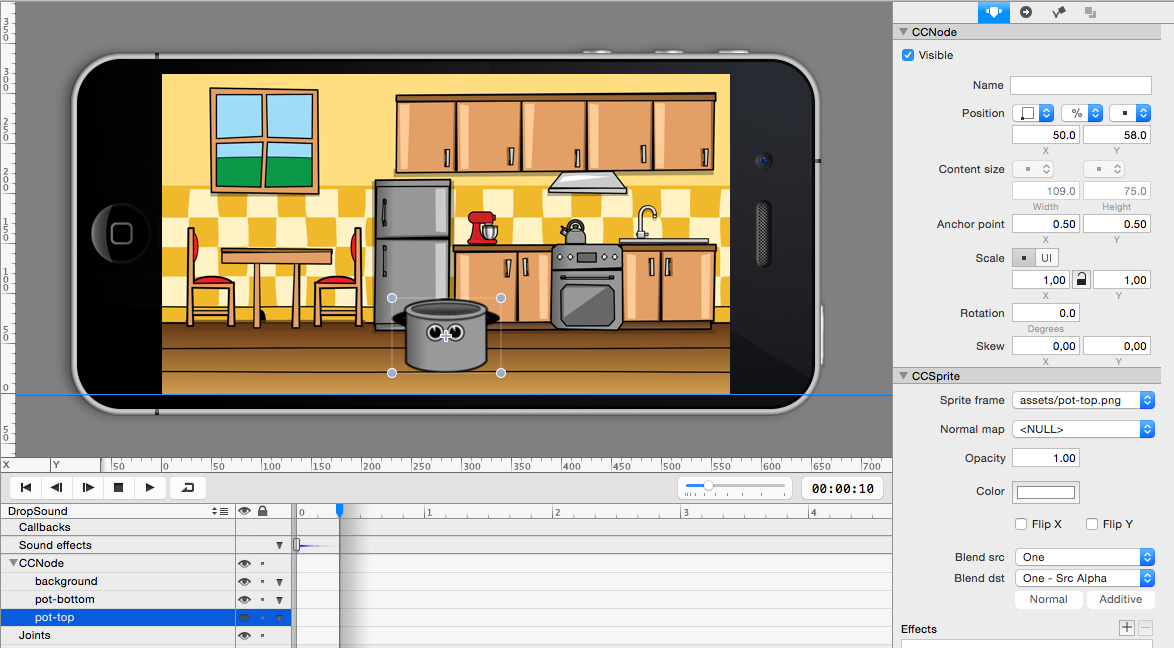
\includegraphics[width=0.9\linewidth]{images/Chapter3/add_pot.png}
		\caption{Add both pot parts to the main scene}
\end{figure}

\begin{leftbar}
The assets of both pot parts have exactly the same dimensions.
 Place both of them at 50\% X position and at a Y position of 58
Create code connections for both pot parts, linked to the \textit{Document Root}. 
Name them \inlinecode{potBottom} and \inlinecode{potTop} respectively.
Publish the \SB{} project
\end{leftbar}

Next, move to the \xcode{} project to set up the code connection variables and
implement the touch handling code.

\begin{leftbar}
Open \inlinecode{MainScene.swift} and add instance variables for our code
connections at the top of the class:
\begin{lstlisting}
weak var potTop:CCSprite!
weak var potBottom:CCSprite!
\end{lstlisting}
\end{leftbar}
There are three important things to remember about these code connections.
Firstly, all code connections should be marked as \inlinecode{weak}.
\inlinecode{MainScene} has a reference to the pot sprites but does not
\textit{own} them. Instead they are owned by their parent node. For any
references that don't mark an ownership, \inlinecode{weak} should be used. 

Secondly, we always want to declare code connections as \textit{forcefully
unwrapped optionals} as denoted by the bang (!) after the type. Swift
requires that all instance variables that aren't optionals are either
initialized with a default value or get set to a value in one of the
initializers of the class, that way the compiler can guarantee that these
variables never contain a \inlinecode{nil} value. Code connections however are
set up after the object is initialized (they are guaranteed to be set up
when \inlinecode{didLoadFromCCB} is called on the node), so technically these
should be optional values. Adding a lot of code for \inlinecode{nil} checking
would clutter our classes, that's why we prefer using the bang notation which
basically says: \textit{I am confident that this value will never be nil when I
am trying to access it}. This is true for code connections as we now that
\cocos{} guarantees to have set them up by the time \inlinecode{didLoadFromCCB}
is called.

Lastly, be careful not to mark these variables as \inlinecode{private}.
Otherwise \cocos{} will not have access to them and won't be able to set up the
code connections.

Okay, now we have the basics set up and are ready to dive into the details of
implementing a drag and drop mechanism!

\section{Implement a Drag and Drop mechanism}
For the very first project in this book we have already implemented a basic
touch mechanism. You should remember that \inlinecode{userInteractionEnabled} is
the property that activates/deactivates touch handling for a node and that
\cocos{} provides four different callbacks for different state transitions in
the lifecycle of a touch. Here's the recap:

\begin{description}
\item[touchBegan:] called when a touch begins
\item[touchMoved:] called when the touch position of a touch changes
\item[touchEnded:] called when a touch ends because the user stops touching the
screen
\item[touchCancelled:] called when a touch is cancelled because user moves touch
outside of the touch area of a node
\end{description}

Knowing that, how can we implement a drag and drop control scheme for our game?
Dragging and dropping includes three different steps:
\begin{enumerate}
  \item Pick up object
  \item Drag object
  \item Drop object
\end{enumerate}

\subsection{Picking up an Object}
In order to pick up an object we need to detect a user's touch and determine if
the touch is within the boundaries of our object, if that is the case,
we start dragging the object.

First of all, let's turn on user interaction for the \inlinecode{MainScene}
class, so that we receive touch events.

\begin{leftbar}
Add the required line to the \inlinecode{onEnterTransitionDidFinish} method:
\begin{lstlisting}
  override func onEnterTransitionDidFinish() {
    super.onEnterTransitionDidFinish()
    
    self.userInteractionEnabled = true
    
    // spawn objects with defined frequency
    schedule("spawnObject", interval: spawnFrequency)
  }
\end{lstlisting}
\end{leftbar}

Next, we need to add the touch handling method. The touch handling method will
need to check if the touch is within our pot. If that is the case, the method
will need to set a state variable that remembers that we are currently dragging
this object. If the user moves a finger across the screen and we are currently
in object dragging mode, it is important that the object follows the finger of
the user.

\begin{leftbar}
Add this implementation to \inlinecode{MainScene.swift}:
\begin{lstlisting}
  override func touchBegan(touch: CCTouch, withEvent event: CCTouchEvent) {
    if (CGRectContainsPoint(potBottom.boundingBox(), touch.locationInNode(self))) {
      isDraggingPot = true
      dragTouchOffset = ccpSub(potBottom.anchorPointInPoints, touch.locationInNode(potBottom))
    }
  }
\end{lstlisting}
\end{leftbar}

Let's discuss this implementation briefly. You already have seen the usage of 
\inlinecode{touch.locationInNode(self)} in the first chapter of this book,
where we briefly discussed touch handling
(\ref{Introduction_FirstTouchHandling}). This method returns the touch position
within a given node. In this specific case we are receiving the touch position
within \inlinecode{MainScene}.

Next, we are using a utility function, \inlinecode{CGRectContainsPoint}, to
check if this touch is within the pot. Remember,
that \inlinecode{potBottom} and \inlinecode{potTop} are placed at exactly
the same position, so we can choose either of them for this check.
\inlinecode{CGRectContainsPoint} takes a rectangle as its first argument and a
point as its second. It returns true if the point is within the rectangle.

If the touch position is inside of the pot, we set our state variable,
\inlinecode{isDraggingPot}, to \inlinecode{true}. 

There is one last line that we didn't discuss upfront:
\begin{lstlisting}
dragTouchOffset = ccpSub(potBottom.anchorPointInPoints, touch.locationInNode(potBottom))
\end{lstlisting}

In order to drag an object smoothly we need to remember where we touched that
object when starting dragging. Take a look at the following diagram:
\begin{figure}[H]
		\centering
		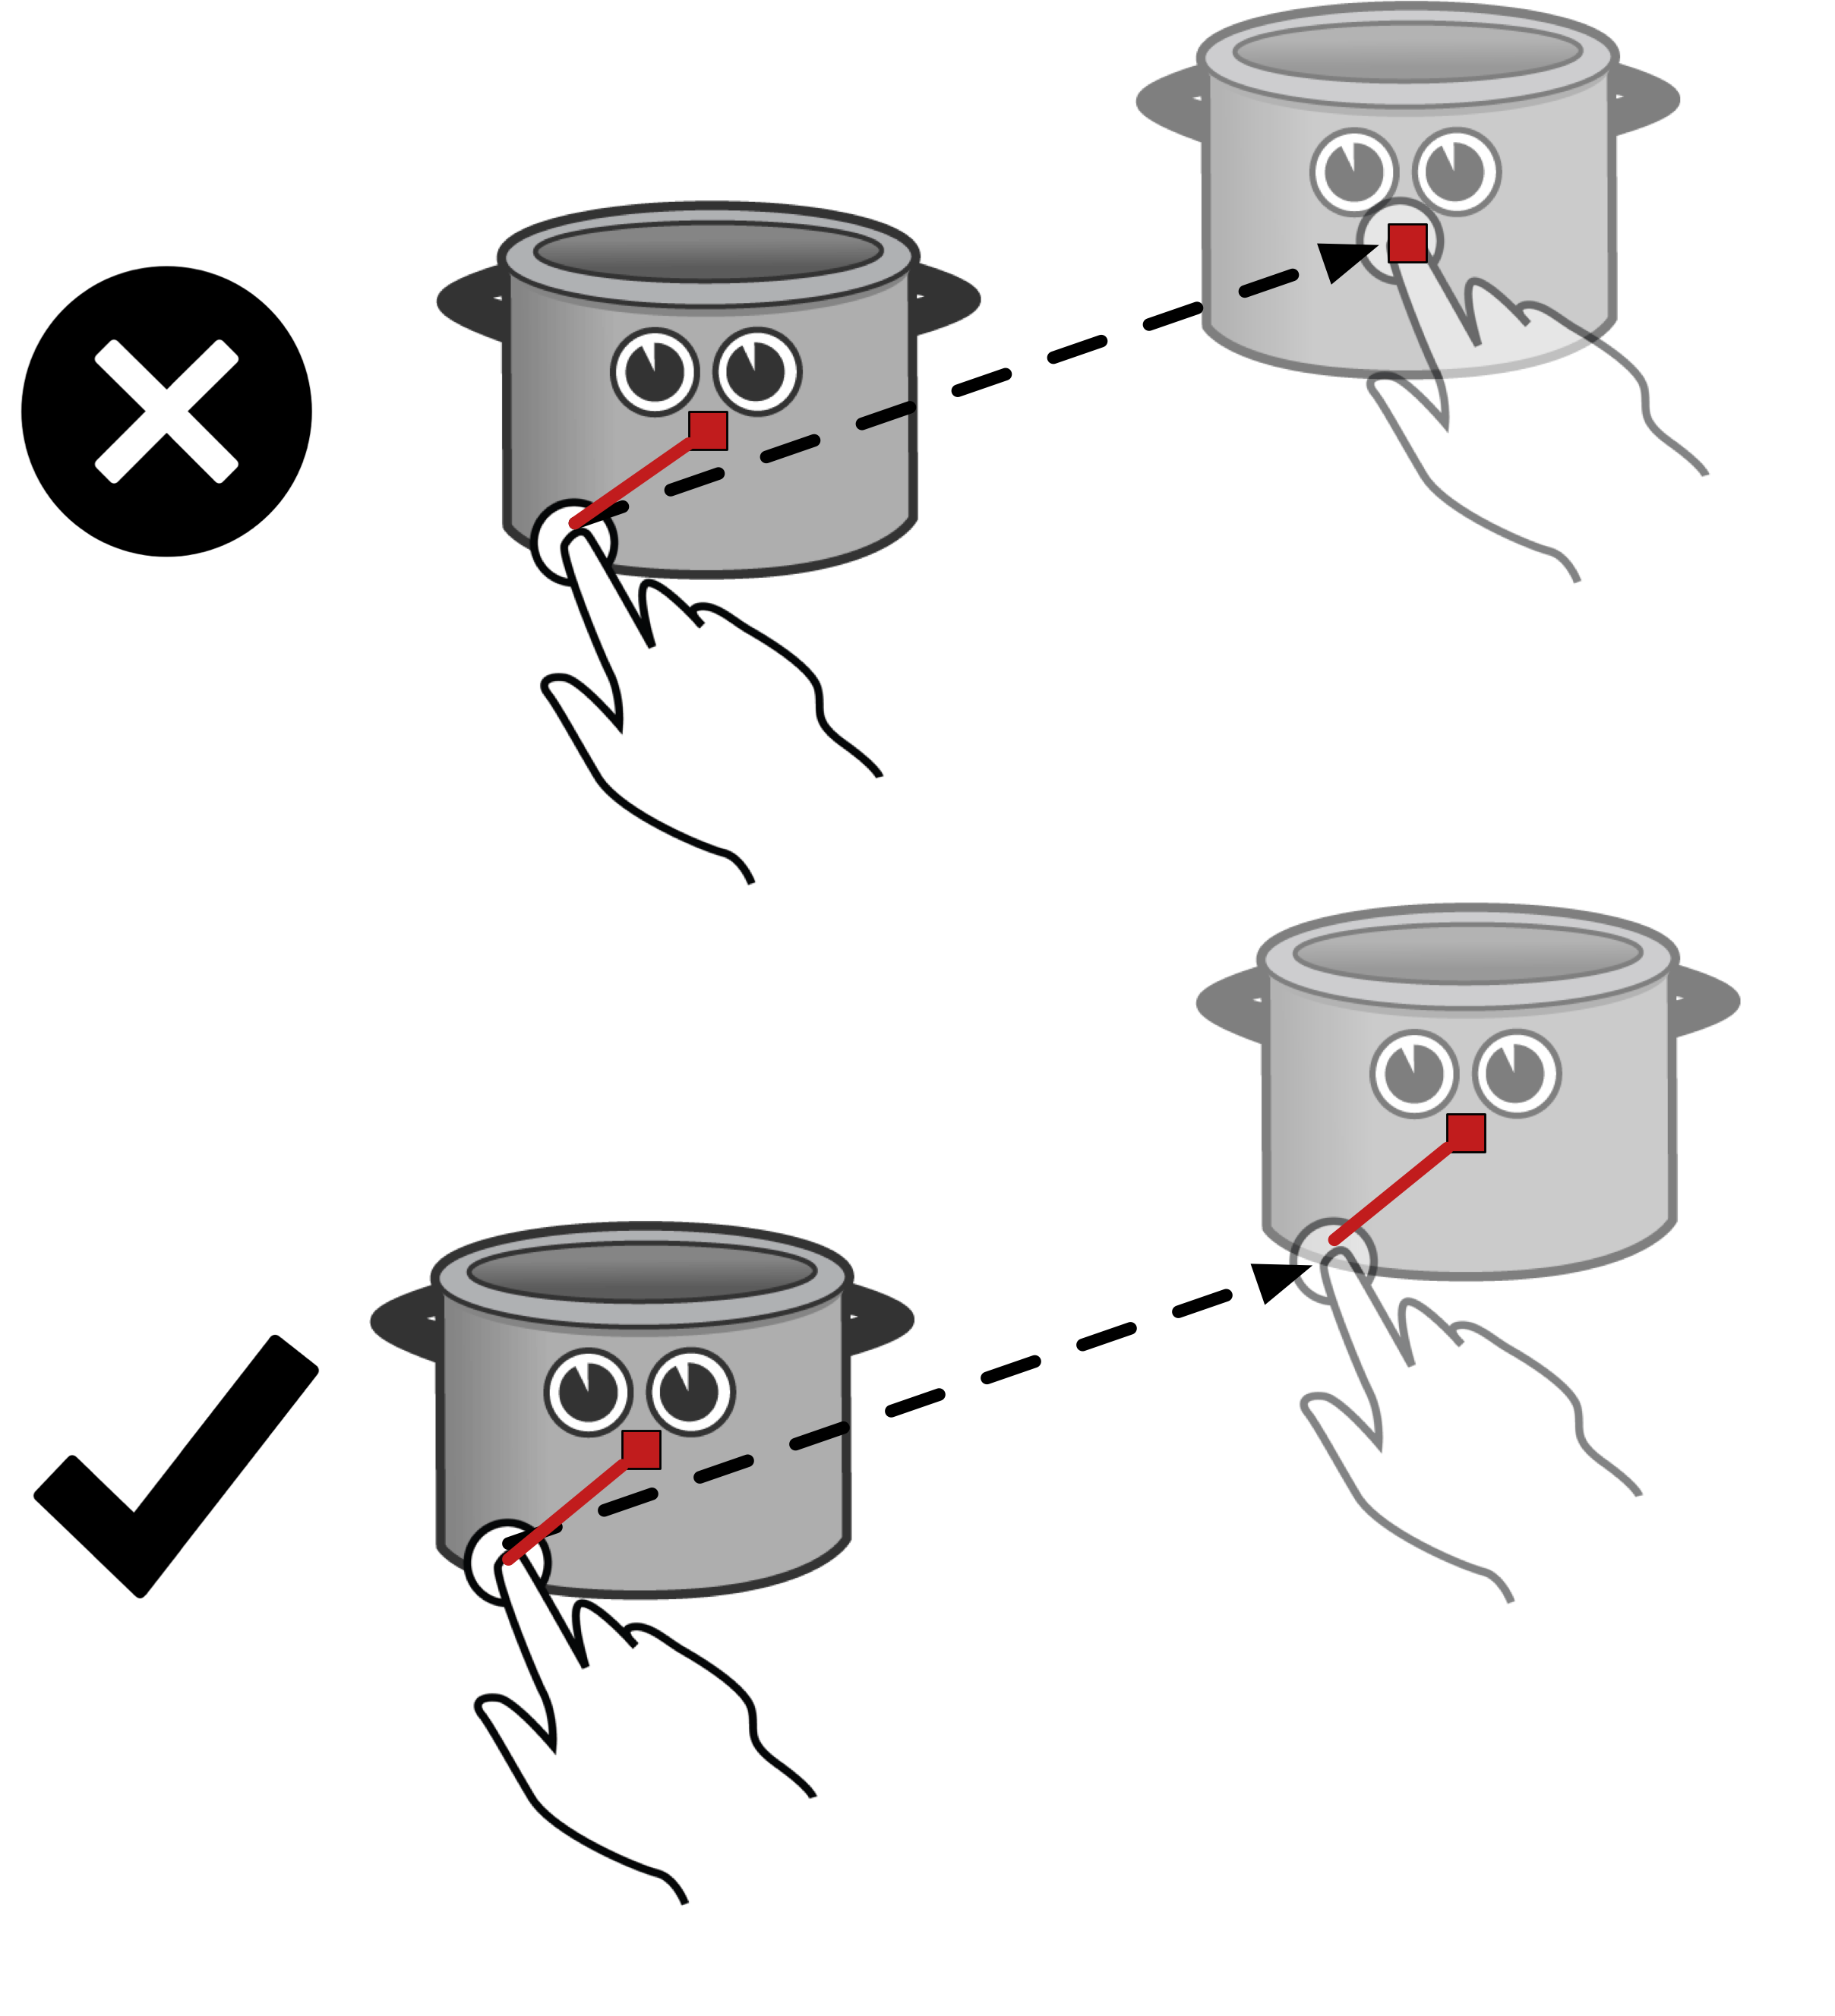
\includegraphics[width=0.4\linewidth]{images/Chapter3/dragging_offset.png}
		\caption{\textit{Top Image:} incorrect implementation, object jumps to touch
		position. \textit{Bottom Image:} correct implementation, touch offset is
		maintained while dragging the object.}
		\label{user_interaction_touch_offset}
\end{figure}
As the user moves the finger, we move the object along. However, the position of
the object is not exactly the touch position. Instead it is the touch position
\textit{plus} the touch offset determined when we started dragging. We determine
that offset by calculating the distance between the anchor point (that's the
reference point for positioning a node, typically it's in the center of the
node) of the touched object and the exact touch position. 
No we know why it is important to store the touch offset!

\begin{leftbar}
To wrap up the implementation of \inlinecode{touchBegan} let's add the two
instance variables we have referenced: \inlinecode{isDraggingPot} and
\inlinecode{dragTouchOffset}. Your list of iVars should now look like this:
\begin{lstlisting}
  weak var potTop:CCSprite!
  weak var potBottom:CCSprite!
  
  private var fallingObjects = [CCNode]()
  private let fallingSpeed = 100.0
  private let spawnFrequency = 0.5
  private var isDraggingPot = false
  private var dragTouchOffset = ccp(0,0)
\end{lstlisting}
\end{leftbar}

\subsection{Moving an Object}
Now we'll implement the code that actually moves the pot. That code needs to run
whenever a user's finger moves. That means we need to implement the
\inlinecode{touchMoved} method.
\begin{leftbar}
Add the \inlinecode{touchMoved} method below the \inlinecode{touchBegan} method:
\begin{lstlisting}
  override func touchMoved(touch: CCTouch, withEvent event: CCTouchEvent) {
    if (!isDraggingPot) {
      return
    }
    
    var newPosition = touch.locationInNode(self)
    // apply touch offset
    newPosition = ccpAdd(newPosition, dragTouchOffset);
    // ensure constant y position
    newPosition = ccp(newPosition.x, potBottom.positionInPoints.y);
    // apply new position to both pot parts
    potBottom.positionInPoints = newPosition;
    potTop.positionInPoints = newPosition;
  }
\end{lstlisting}
\end{leftbar}
In the first line we check if we are currently in dragging mode. If not, we do
nothing and return immediately. This prevents the pot from jumping to the latest
touch position if it has not been picked up beforehand.

If we are in dragging mode we continue. First we get the new touch position.
Then we apply the offset that we discussed in figure
\ref{user_interaction_touch_offset} to that new position. The next line ensures
that the y position of the pot stays constant, we want to allow horizontal
movement only. Finally, we apply that new position to both pot parts. Great,
we're pretty close to finishing the drag and drop functionality.

If you test the app in the current state you'll see that there's one simple yet
important step missing\ldots

\subsection{Dropping an Object}

